%\documentclass[11pt]{article} % use larger type; default would be 10pt
%\usepackage[utf8]{inputenc} % set input encoding (not needed with XeLaTeX)
%
%%%% PAGE DIMENSIONS
%\usepackage{geometry} % to change the page dimensions
%\geometry{a4paper} % or letterpaper (US) or a5paper or....
%\newcommand{\tab}{\hspace*{2em}}
%
%%%% PACKAGES
%\usepackage{graphicx} % support the \includegraphics command and options
%\usepackage{wrapfig} % Figure wrapping
%% \usepackage[parfill]{parskip} % Activate to begin paragraphs with an empty line rather than an indent
%\usepackage{booktabs} % for much better looking tables
%\usepackage{array} % for better arrays (eg matrices) in maths
%\usepackage{paralist} % very flexible & customisable lists (eg. enumerate/itemize, etc.)
%\usepackage{verbatim} % adds environment for commenting out blocks of text & for better verbatim
%\usepackage{subfig} % make it possible to include more than one captioned figure/table in a single float
%\usepackage{url}
%\usepackage{enumerate}
%\usepackage{cleveref}  %cites figures intelligently
%\usepackage{import} % document structuring
%\usepackage{float}  %These two ensure that table position follows text by specifying {table}[H]
%\restylefloat{table}
%
%%\usepackage[T1]{fontenc} % Enables foreign symbols
%
%%CODE LISTINGS
%\usepackage{color}
%\usepackage{listings}
%
%\lstset{
%	tabsize=4,
%%	language=matlab,
%        	basicstyle=\scriptsize,
%%     	upquote=true,
%       	aboveskip={\baselineskip},
%        	columns=fixed,
%        	showstringspaces=false,
%        	extendedchars=true,
%        	breaklines=true,
%	prebreak = \raisebox{0ex}[0ex][0ex]{\ensuremath{\hookleftarrow}},
%	frame=single,
%        	showtabs=false,
%        	showspaces=false,
%        	showstringspaces=false,
%        	identifierstyle=\ttfamily,
%        	keywordstyle=\color[rgb]{0,0,1},
%        	commentstyle=\color[rgb]{0.133,0.545,0.133},
%        	stringstyle=\color[rgb]{0.627,0.126,0.941},
%	language=C++
%}
%
%%%% HEADERS & FOOTERS
%\usepackage{fancyhdr} % This should be set AFTER setting up the page geometry
%\pagestyle{fancy} % options: empty , plain , fancy
%\renewcommand{\headrulewidth}{0pt} % customise the layout...
%\lhead{}\chead{}\rhead{}
%\lfoot{}\cfoot{\thepage}\rfoot{}
%
%%%% SECTION TITLE APPEARANCE
%\usepackage{sectsty}
%\allsectionsfont{\sffamily\mdseries\upshape} % (See the fntguide.pdf for font help)
%\usepackage{titlesec}
%%\titleformat{\subsection}[runin]{\mdseries\bf}{\thesubsection}{1em}{}
%%\titleformat{\subsubsection}[runin]{\mdseries\bf\underline\large}{\thesubsection}{1 em}{\vspace{-5 pt}}
%
%% (This matches ConTeXt defaults)
%
%%%% ToC (table of contents) APPEARANCE
%%\usepackage[nottoc,notlof,notlot]{tocbibind} % Put the bibliography in the ToC
%\usepackage[titles,subfigure]{tocloft} % Alter the style of the Table of Contents
%\renewcommand{\cftsecfont}{\rmfamily\mdseries\upshape}
%\renewcommand{\cftsecpagefont}{\rmfamily\mdseries\upshape} % No bold!
%
%\begin{document}

\part{TimeLapse}
Time-lapse photography is the process by which a camera is set up to watch a particular object for extended periods of time. Instead of the camera taking frames continuously for that period, intervals are specified which are much lower than the normal framerate (e.g. 1 frame per hour). Once the frames are accumulated and played at a normal frame rate (e.g 30 frame per second) then time appears to run fast and lapsing occurs.
The technique has been used to capture crowds of people, traffic, and other everyday entities which at a normal speed seem unimpressionable, but at high speeds become a fast flurry of activity.

There were three approaches I could take to make a TimeLapse application:\\
\begin{enumerate}
\vspace{-20pt}
\item Run the app continuously for the full duration of the time lapse period specified.\\
\vspace{-20pt}
\item Run the app continuously in the background for the full duration of the time lapse period.\\
\vspace{-20pt}
\item Schedule the app to run and exit at specified times until the full duration of the time lapse period\\
\vspace{-10pt}
\end{enumerate}

The first approach would have meant that the application would have been in the main foreground while all the frames were being taken. If I wanted to capture a frame every hour for two days, then the app would have to be open and active for that entire time. This would be a waste of RAM, since the application will occupy a chunk of memory for two days without actually doing any work for most of that time. This will also occupy window space since the application UI will be active in this time, which is a major problem because the user may unwittingly close the application preventing it from completing it's job.

The second approach is the same as the first; waste of RAM over an extended period of time, but this time the window of the application is hidden and so the user will not be able to accidentally cancel the task once it is set. Doing this is very easy, since in Qt all one has to do is get rid of the myClass->show() function to run the app in the background. But as before, this is not optimal and wastes RAM.

This leaves the third option, which is to set scheduled events for the app so that it starts and stops at specific times with minimal usage of system resources. The question now is how to enable the MotionDetector to do this.

\section{Command Line Switches}

Commandline switches enable the user to issue commands to a program through a line of text. It is essentially a text-based user interface and the user can specify the level of control through arguments, which are extra text appended (with spaces) to the program name. By convention 'flags' or 'switches' are often used which specify arguments using dash or double-dash notation such as '--flag'.

\subsection{Argument parser}

Qt (like most SDk's) places all the arguments to a program in a list of some kind. In Qt, the arguments are accessed via QApplication::arguments() which returns the arguments in a QStringList (very similar to an ArrayList in Java).

My first step was to create a CommandLine class. This class would take a reference to the QStringList and check the tokens within that for certain key flag values. The key flag values needed would have to be same options that can be specified by the user, and so I settled with the standard convention of providing longhand and shorthand names for flags with '- -name' and '-n' respectively:
\begin{frame}{}
\lstinputlisting[title=\textbf{Source Code: help.sh}]{../Code/commandline/help.sh}
\label{frame:help}
\end{frame}

To search for flags, I used QStringLists' ".contains(key)" method which performs a search over all the tokens in the argument list. This can be very slow, especially if other less important flags are searched first. 
For this reason, flags such as '--help' or '--version' were the first two flags to be searched, since these will print a quick message and then terminate without having to check for further flags.

The other flags followed a different logic:
\begin{frame}{}
\vspace{-10pt}
\lstinputlisting[title=\textbf{Source Code: checkflag.cpp }]{../Code/commandline/checkflag.cpp}
\end{frame}
 First a default value would be set (in this case 5) for the flag\_value, then a search would commence within the if statement.  The '.indexOf(key)' method would find the index of the flag in the array, or else return -1 if not found. I followed the convention where I would first check for the shorthand name first, and then the longer one since I reasoned that it was less effort to type a shortflag than a longer one, and was thus more likely to occur. This is useful, since C++ supports short-circuit evaluation and so if the first condition is deemed true, it will not need to search the other end of the OR statement.

The flag\_value is then assigned the integer (or other type) version of index after the flag (e.g. We want to grab the 3 from the argument '--flag 3'). In Qt, this is returned as 0 if it could not convert it properly and so some error checking needs to be performed.

\subsubsection{Switch Detection}
Once the flag has had all the useful arguments taken from it, it is then {\it removed} from the argument array in order of highest index for flag, to lowest index for flag (the flag name). This order is necesary because when you remove from an Array at a certain index, all the indexes above it are shifted down meaning you now have to subtract by 1 to access a certain item from the higher indexes which can lead to errors. It is therefore far easier to remove from high index to low index to ensure that the lower indexes are unaffected by changes in the higher indexes.

Why is removal even important here? It's an optimization. By removing the arguments from the array after using them, future searches to that same array for different flag values will be {\it faster} because there are less items to check. This also gives another benefit in that if the user misspells or enters an unknown flag, it will be left over in the argument array , and so the program can notify the user precisely of which flags were not recognised and which one's were:
\begin{frame}{}
\lstinputlisting[title=\textbf{Source Code: unknowns.cpp }]{../Code/commandline/unknowns.cpp}
\end{frame}

So if the user types into a shell:\\
\tab' motiondetect -m 7 --size 320 240 --roger the dodger -w 100'\\
The app will spit out the following error:\\
\tab'Could not parse: --roger the dodger\\Please try --help for more info '

since these will be the leftover arguments that were left in the argument list. Had all the flags been valid, the argument list would have been empty.

Some flags rely on other flags such as '--delete' and '--convert'.  Delete specifies that the images should be deleted after all operations complete, and Convert specifies that the images should be converted to a movie after all operations complete. 
If the user wishes to convert the images after completion, then they are free to choose to delete or not to delete. But if they wish to simply delete without first converting, then an error pops up highlighting how pointless the operation will be - since it will be taking photos and then deleting them after.

\paragraph{Terminal Colours\\}{
To make the commandline look as interesting as possible I also implemented colours into the shell. Fremantle uses the busybox shell by default, which is a lightweight shel that comes prepackaged with many standard utils such as 'ls' 'mv' 'cp' and so forth which are symlinked to /usr/bin/ so as to appear independent of busybox.
Busybox also shares the same as terminal colour codes as Bash, which are called via non-printing escape sequences which are enclosed in \textbackslash[\textbackslash033[ and \textbackslash] pairs.
Using the following colour codes in \cref{tab:colorcodes}, different colours could be printed

\begin{table}[H]
\centering
\begin{tabular}{| r | l |}
\hline
\multicolumn{2}{|c|}{\bf Color codes} \\
\hline
char red[ ] &"\textbackslash033[0;31m\textbackslash033[1m"\\
char cyan[ ] &"\textbackslash033[0;36m"\\
char yellow[ ] &"\textbackslash033[0;33m"\\
char green[ ] &"\textbackslash033[0;32m"\\
char stop[ ] &"\textbackslash033[0m"\\
\hline
\end{tabular}
\caption{Red is a longer sequence than the other colours because default red was not very visible, so I made it {\bf bold} too by appending \textbackslash033[1m" to it.}
\label{tab:colorcodes}
\end{table}

With these codes I could then control what colours I wanted to use by simply calling:\\
cout  yellow \(\langle\langle\) "Warning:" \(\langle\langle\) green \(\langle\langle\) "This shell supports" \(\langle\langle\) cyan \(\langle\langle\) "multiple"\(\langle\langle\)  red \(\langle\langle\) "colors!" \(\langle\langle\) stop \(\langle\langle\) endl;

The stop colour at the end is neccesary to reset the shell to its default color, otherwise the last color set will be maintained for the next message which may not be desirable.

\begin{figure}[H]
	\vspace{-10pt}
	\begin{center}
		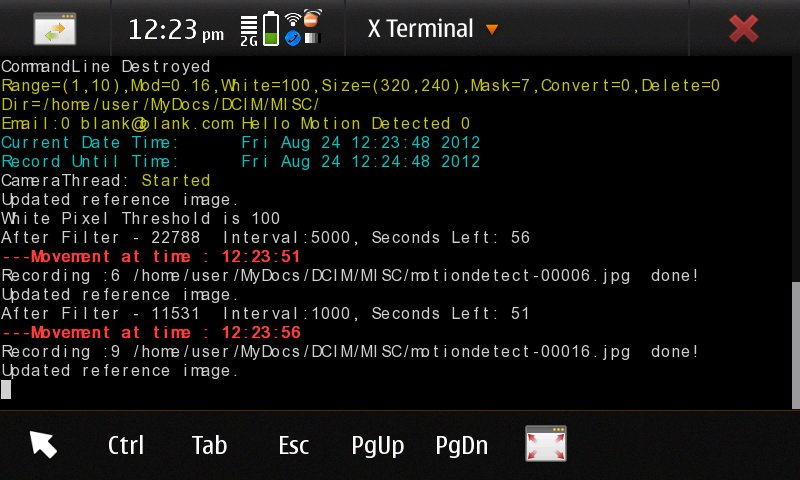
\includegraphics[width=0.8\textwidth]{../images/commandline/commandscreen.jpg}
	\end{center}
	\vspace{-20pt}
	\caption{Screenshot fom phone}
	\label{img:command}
	\vspace{-10pt}
\end{figure}

One of the main benefits of having a commandline implementation is that enables remote usage. A user can simply ssh or telnet into the phone from another machine and start and control the application from the shell on their own computer. The colours will also print correctly too.

{\small\bf It should be noted that at this stage std::cout replaced qDebug, the default Qt output stream, and message handlers are also attempted in order to enable verbose output for commandline. The implementation attempt for this is detailed on page~\pageref{qdebug} in the Other Implementations section of the Appendix.}

}
\subsubsection{Reusing existing variables}

For standard motiondetection commandline calls such as mask, whitepixel, size, etc as shown in help.sh on page~\pageref{frame:help}, individual variables were created to hold these values, which were mirror variables for the same ones in the CameraThread. When the Commandline finishes parsing arguments it switches flow control back to the motiondetector (main window UI) class which then reassigns these variables to those of the camerathread as shown below:
\begin{frame}{}
\lstinputlisting[title=\textbf{Snippet from MotionDetector (mainwindow UI) }]{../Code/commandline/commandtoops.cpp}
\end{frame}
The main MotionDetector class does not have variables in the header file that hold all the variables, like CommandLine and Operations (the camera thread) do. MotionDetector is simply a UI class, it acts as a waypoint or a go-between for connecting commandline arguments to the camerathread.

When commandline arguments are not given, the 'commands' pointer is initialised to zero and is thus empty. In this case the UI is active and so Operations gets its values directly from the UI. When the pointer is not empty, the UI is ignored and Operations gets its values directly from CommandLine. An exit slot is also connected in this case, so that when the camera thread finishes, the entire application safely closes (which overrides the default finish behaviour, where the UI simply becomes active and listens for input again).

The real trick is when we want to perform a timelapse operation. Timelapse operations need only five arguments:
\\ Image width, frame rate, convert images to movie,  delete images after conversion, and end date.\\
(height does not need to be specified since it can be inferred from width, reducing the number of neccesary arguments).\\
Image width, convert and delete are variables used in motiondetection operations, so these values can be assigned correctly. But what do we do with frame rate and end date? These variables do not exist for motion detection operations, and it would be wasteful to create new variables for them, because as discussed above; whatever variables we create in commandline we must also create in Operations (the camera thread). Creating a framerate and enddate variable will be making variables that will be unused most of the time.

Instead, we reuse the one's that exist already but are not being used. To pass framerate into operations, we simply pass it as a mask variable (they are both integers) and to pass the end date we pass it as a time variable that is normally used in the motiondetector as duration. This reduces the number of class variables and in turn reduces overhead.

This maybe frowned upon in certain circles due to the error prone nature of using a single variable for multiple different operations, but as long as it is done safely it is much more efficient. In this case, the camera thread needs to know whether the operation it is about to perform is a motion detection or a time lapsing one, and so a timelapse boolean had to be created. This may seem like a step backwards after what I just said about reusing variables, but it is neccesary because for a motion detection operation all the other variables will be used up, plus this ensures that should I wish to create further options for the timelapse part of the app I can just slot them into the currently inactive motiondetector variables.

\section{Scheduled Events}

Scheduled events are events that have been schedules to run at specific times. They are often used to automate system daemons, but can also be acessed by the user to run scripts or programs at specific times.

\subsection{Cron}\label{cronalarm}
In Linux 'cron' is the job scheduler, and it performs its operations by reading from a 'crontab' file which is a configuration file detailing the date and frequency, and job-specific detail of the job.

Cron jobs are prepended by an intuitive 5 character sequence which is used to define the date and frequency via:\\
\begin{figure}[H]
\vspace{-20pt}
	\begin{center}
		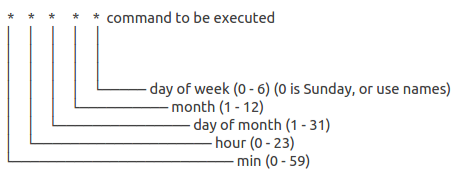
\includegraphics[width=0.7\textwidth]{../images/cron}
	\end{center}
	\vspace{-20pt}
	\caption{Cron example from Wikipedia}
	\vspace{-10pt}
\end{figure}


\begin{table}[H]
\centering
\begin{tabular}{| l | l |}
\hline
\multicolumn{2}{|c|}{\bf Quick Crash Course in Crontabs} \\
\hline
Run every minute for eternity:  &  *\tab*\tab*\tab*\tab*\\
Run at 11am and 2pm every day:& 0\tab 11,14\tab*\tab*\tab*\\
Run every mon,tue, wed,fri at 12 pm every 10 mins:&   */10\tab 12\tab*\tab*\tab1-3,5\\
Run at 8:14 and 8:15 every October 21st that is a Tuesday& 14,15\tab 8\tab21\tab*\tab2\\
\hline
\end{tabular}
\caption{Cron tab examples}
\label{tab:cron}
\end{table}

So to run out motiondetection application every alternate winter morning at 8am, I would set a cronjob as:\\
' \tab*\tab8\tab*/2\tab12,1,2\tab*\tab  motiondetect --my-flag'

\subsection{TimeLapse hidden command flag/switch}

The importance of the commandline functionality mentioned in the previous section was to ensure that the app could be issued a command that would enable it to run and exit by itself. For scheduled events this would mean using a specific flag to issue time lapse operations.

This flag is hidden from the user (i.e. it is not documented in the help text as shown on page~\pageref{frame:help}. This is because it is the app itself that sets the scheduled event, and not the user. The user should not be able to set a scheduled event accidentally/maliciously from the commandline.

To ensure this I made the flag for running the timelapse operations an obscure mix of two words that are normally not likely to be next to each other in a given sentence:\\
'motiondetect --teenage-diplomacy \(\langle\)DateTime\(\rangle\) \(\langle\)Convert\(\rangle\) \(\langle\)Delete\(\rangle\) \(\langle\)Width\(\rangle\) \(\langle\)fps\(\rangle\)'. This is a reference to 'Blinded By the Light' song by Bruce Springsteen later covered by ELO. I figured no one would actually use that as a command call.

The code is as follows:
\begin{frame}{}
\lstinputlisting[title=\textbf{Snippet from CommandLine.cpp}]{../Code/commandline/secrettime.cpp}
\label{code:secret}
\end{frame}

As you can see  the error/exit messages of the function call arent very informative either with an unhelpful "Nice Try" error message whenever the arguments aren't of the right length or format. 

\subsubsection{Logic of repeated calls}

The snippet of code shown on page~\pageref{code:secret} shows how to call the timelapse operation. This function is called repeatedly for scheduled events, and it is called with the same arguments every time for each task set. This might seem somewhat counterintuitive to be using the same DateTime value for each job within a task but the logic is sound:

\begin{enumerate}
\item I set a DateTime value for 10th October 2012 3pm (the date I want the task to end.)  I set an image size of 320x240.\\
\vspace{-20pt}
\item I set that I want it to convert the images to a movie on completion, and that I want the the images deleted. I set a fps of 25.\\
\vspace{-20pt}
\item I set an interval of 30 minutes for how often I want to set a job until it terminates at the DateTime value I set in the previous step.\\
\vspace{-20pt}
\item The app sets jobs to the scheduler specifying that the system should run:\\
 ' motiondetector --teenage-diplomacy 10:10:2012:15:00:00   1  1  320 25' \\
every half hour until 10th October 2012 3pm.
\vspace{-8pt}
\item When the app executes using this flag, it compares the {\it current DateTime} with the end DateTime. If the current is less than the end, then it takes a photo using the size parameter and exits. Otherwise if the current date is {\it later} than the end date, it knows to convert (at 25 fps), delete, then exit.
\end{enumerate}
All this, purely by using the same argument values.

\section{Available Software Evaluation}
In order to get repeated application calls in the first place, we need to first schedule the jobs. Fremantle uses cron (as do most systems), but it also has it's own native scheduler daemon 'Alarmd'.

\subsection{Cron vs Alarmd}
\subsubsection{Cron}

Cron is native to all Linux-based OS's and to set a job, one has to edit /etc/cron.daily/(add item here).  A job is added as a cron string with a command appended and it is the duty of the user to remove the string when that job is to terminate. To do this, the app must read all jobs from the file and filter out which ones belong to the application and which ones dont, then check to see if any of them require retiring, and if so removing them. This is doable, but very pinneckety.

Unfortunately this is seen as somewhat risky, and can lead to unpredictable behaviour, mostly because cron is only used on the device for system specific actions (such as /etc/cron.daily/locate which periodically updates the phone's tracker for media files), so any custom user-specific actions are somewhat temperamental.  I therefore had to abandon cron and look for something else.

\subsubsection{Alarmd}
Alarmd is a Maemo-native system daemon that {\it manages} queued alarm events which "executes actions defined in events either automatically or after user input via system ui dialog service"\footnote{Alarmd Maemo Package - http://maemo.org/packages/view/alarmd/}\label{ref:alarmdpack}. At first glance it may seem like a front-end for cron, but by checking the dependencies it is seen that it talks directly to dbus. DBus is a low-level inter-system messaging/communication system for making system calls between applications, that it has been so well-engrained in Linux operating systems that it has only a single dependency.

Alarmd is commonly used by the system to manage making multiple wake up alarms, but it is not restricted to that function and technically can be used to execute any alarm at any given time. It has a much easier API then cron, and does a lot of useful scheduling background tasks by itself such as removing a job from the list once complete. 

In alarmd, jobs are contained between three objects: Cookies, Events, and Actions.
\begin{description}
  \item[Cookies] ID for the job. Can be cast as a long, and cast back into a cookie\_t object
  \item[Actions] This describes what the alarm will do when it is called, and how it is called. It has two triggers (event listeners): Type triggers and When Triggers.
\begin{enumerate}
\item Type triggers determine what functionality the alarm has and common types are ALARM\_ACTION\_WHEN\_TYPE\_SNOOZE (snooze button that offputs the alarm for 10 more minutes) but for executing commands, the trigger I was using was ALARM\_ACTION\_TYPE\_EXEC. 
\item When triggers determine the context in which the alarm will be triggered. Common types are ALARM\_ACTION\_WHEN\_RESPONDED but I was using ALARM\_ACTION\_WHEN\_TRIGGERED.
\end{enumerate}
Triggers have hex values, and an action is usually performed as a bitwise OR pair of Type and When triggers:\\
'act-\(\rangle\)flags \textbar= (ALARM\_ACTION\_WHEN\_TRIGGERED \textbar ALARM\_ACTION\_TYPE\_EXEC)';\\
which performs bitwise OR upon these two triggers and sets the flag to "'true'" when one of these is satisfied.
 \item[Events] These are containers for Actions, and are what Alarmd holds. To add an alarm to Alarmd, you add an 'Event'. Events also hold the time\_t for the alarm, and has support for  seconds, something that cron does not have.
\end{description}

To use Alarmd, one needs to use libalarmd, which is native to the phone and so the rootstrap device already had it installed. The class I created borrowed the template for a few of it's functions from the examples at the Maemo Wiki\footnote{Alarmd Framework -- http://wiki.maemo.org/Documentation/Maemo\_5\_Developer\_Guide/Using\_Generic\_Platform\_Components/Alarm\_Framework}
\label{ref:alarmdframe}. 
Alarmd jobs have APPID's, which uniquely match a job to an application making it far easier to retrieve and edit jobs without affecting other jobs or having to filter through them.

\section{Optimisations/Error Proofing}
Commandline not called until arguments!=0, then it is destroyed intelligently.

Even with the decent examples at the Maemo wiki, the application was error prone: sometimes jobs would be added correctly and sometimes not, sometimes the jobs would execute correctly and sometimes not. 

This was actually one of the most longest bugs to fix due to the temperamental nature of the errors. I eventually did find a fix by searching through the source code {\it Alarmed\footnote{Alarmed python package and source - http://maemo.org/packages/view/alarmed/}\label{ref:alarmedpyth}}, a python GUI for adding alarmed events to the scheduler using python bindings for libalarmd. The syntax was much the same and very soon I realised that the error turned out to be a problem with alarmd running commands from busybox, but should instead be running them from the Ash shell by prepending '/usr/bin/ash' to the executed strings. The app added and executed events flawlessly after that stage.

\subsection{Kill Switch}


Another problem that occured early on was accidentally setting the interval to every second. I did this to my mistake and was greeted by a "hello" prompt every second for at least 10 minutes while I simultaneously killed each process ID matching the alarm, and deleted each alarm individually from the app. That was a quick lesson I learned: Always have a kill switch.

First I created a button that deleted {\it all} alarmd jobs for the application, and then I created a function that killed all process ID's matching a timelapse operation from the shell. The call I made was:\\
\vspace{-20pt}
\begin{lstlisting}[title=Kill Function]
void killAllOccurencesOfApp(){
    QStringList pids = terminalAction("ps aux | grep teenage\\-dipl | awk '{print $1}'", true).split('\n');
    QString kill = "echo 'kill ";
    for (char i=0; i< pids.length(); i++)
    {
        kill.append(pids.at(i)+" ");
    }
    kill.append("' | root");
    std::cout << "Command: " << kill.toUtf8().data() << std::endl;

    terminalAction(kill);
\end{lstlisting}
The function prints a list of all active processes and greps the lines where 'teenage-diplomat' match, then pipes the output into awk which grabs the first column (containing the PID's) and splits them into an array. Then a kill command is issued by appending the contents of the array into a string and run as root.

The kill switch is a hidden function; it is not to be used lightly and so there is not one button that calls it. Instead it is activated by a sequence of button pressed in succession each other. This is to enable that it is not accidentally pressed by the user, but is only used in emergencies.

Setting the interval to less than 30 is not permitted either, but this is discussed later in the User Interfaces Section on page~\pageref{userinterfaces}.

\subsection{Easter Egg}
Also included in the commandline is a small easter egg that launches a Asteroids/Snake game I wrote using the curses library in python. It was written in between journeys to UCL and home during the development and writeup, and it felt like a shame to leave it out out of the app.
It was written on the phone itself, using the nano text editor.

To access it, the user must type 'motiondetect --easter'. The code can be found on page~\pageref{easter} in the Appendix.

\begin{thebibliography}{9}
\bibitem{alarmdpack}
Simo Piiroinen, Alarm Daemon,  Source: \url{http://maemo.org/packages/view/alarmd/}
Page~\pageref{ref:alarmdpack}

\bibitem{alarmedpyth}
Carol Alexandru, Alarmed Scheduling Application Package and Source - \url{http://maemo.org/packages/view/alarmed/}
Page~\pageref{ref:alarmedpyth}

\bibitem{alarmdframe}
Maemo Documentation Wiki, Alarmd Framework - \url{http://wiki.maemo.org/Documentation/Maemo_5_Developer_Guide/Using_Generic_Platform_Components/Alarm_Framework}
Page~\pageref{ref:alarmdframe}

\end{thebibliography}


%\end{document}